\documentclass[a4paper,11pt]{article}
\usepackage[vietnamese]{babel}
\usepackage{enumerate}
\usepackage{enumitem}
\usepackage{tabularx}
\usepackage{booktabs}
\usepackage{amsmath}
\usepackage{booktabs}
\usepackage{booktabs} 
\usepackage{tabularx}
\usepackage{graphicx}
\usepackage{float}
\usepackage{enumitem} % Tiện tay khai báo luôn cái này để không bị lỗi danh sách (itemize)
\begin{document}\begin{titlepage}
    \begin{center}
        % --- PHẦN HEADER & LOGO ---    
        {\Large \textbf{ĐẠI HỌC BÁCH KHOA HÀ NỘI}} \\[0.2cm]
        {\Large \textbf{KHOA TOÁN - TIN}} \\
		\rule{0.6\textwidth}{1pt}\\[0.5cm] % Đường kẻ ngang trang trí
            \begin{center}
                
\includegraphics[width=0.2\textwidth]{IMG/HUSTLOGO.png}
            \end{center}
         
        \vspace{0.5cm}
        % --- PHẦN TÊN BÁO CÁO ---
        {\Huge \textbf{BÁO CÁO MÔN HỌC}} \\[1cm]
        {\Large{HỆ HỖ TRỢ QUYẾT ĐỊNH}}\\[0.5cm]
        {\Large \textbf{Mã môn học: MI4216}} \\[0.5cm]
        
        % Tên đề tài (Bạn có thể chỉnh sửa lại nếu cần)
        {\Large \underline{\textbf{Đề tài:}}}
        {\Large \textbf{Mô hình phân lớp hành vi mua hàng của khách}}
        
        \vspace{2cm}
        
        % --- PHẦN THÔNG TIN GIÁO VIÊN & SINH VIÊN ---
        % Sử dụng bảng để căn lề cho thẳng đẹp
        \large
        \begin{tabular}{l l}
            \textbf{Giáo viên môn học:} & \textbf{TS. Trần Ngọc Thăng} \\[0.3cm]
            \textbf{Sinh viên thực hiện:} & \textbf{Hoàng Mạnh Đức} \\
            \textbf{Mã số sinh viên:}     & 20237311\\ % Điền MSSV của bạn vào đây
            \textbf{Lớp:}                 &  169316
        \end{tabular}
        
        \vfill % Đẩy phần ngày tháng xuống cuối trang
        
        % --- PHẦN FOOTER ---
        \rule{0.4\textwidth}{0.5pt} \\
        \vspace{0.2cm}
        {\large \textbf{Hà Nội, Tháng 04 năm 2026}}
        
    \end{center}
\end{titlepage}

\tableofcontents
\newpage
\listoffigures
\newpage

% 3. Tạo trang Danh mục bảng
\listoftables
\newpage
\section{Giới thiệu bài toán}

\subsection{Bối cảnh}
Trong kỷ nguyên số hóa, Thương mại điện tử (TMĐT) đang trải qua giai đoạn bùng nổ, thay đổi hoàn toàn thói quen mua sắm của người tiêu dùng. Tuy nhiên, một nghịch lý đang diễn ra trong ngành bán lẻ trực tuyến: Lượng truy cập (Traffic) nền tảng rất cao, nhưng tỷ lệ chuyển đổi (Conversion Rate) lại thấp. Theo các báo cáo ngành, tỷ lệ "bỏ rơi giỏ hàng" (Cart Abandonment Rate) trung bình lên tới gần 70\%. Cùng lúc đó, các hệ thống TMĐT lưu trữ một lượng dữ liệu khổng lồ dưới dạng Nhật ký sự kiện (Event Logs), ghi lại từng cú click chuột của khách hàng. Đây là cơ sở dữ liệu quan trọng để ứng dụng Học máy nhằm "đọc vị" ý định của người dùng trong thời gian thực.

\subsection{Lý do chọn đề tài}
Đề tài \textbf{"Dự đoán ý định mua hàng của người dùng trên nền tảng Thương mại điện tử"} được lựa chọn dựa trên hai động lực chính:
\begin{itemize}[itemsep=4pt, leftmargin=*]
    \item \textbf{Về mặt kinh doanh:} Các chiến dịch Marketing hiện tại thường phân phối mã giảm giá đại trà, gây lãng phí ngân sách và giảm biên lợi nhuận. Việc dự đoán chính xác ai sẽ mua hàng giúp doanh nghiệp tối ưu hóa chi phí và chuyển hướng sang Marketing cá nhân hóa (Targeted Marketing).
    \item \textbf{Về mặt kỹ thuật:} Khai thác dữ liệu sự kiện thô (Raw Event Logs) là một thách thức lớn đối với bài toán Học máy. Quá trình này đòi hỏi kỹ thuật trích xuất đặc trưng (Feature Engineering) phức tạp để chuyển hóa hành vi lướt web thành các chỉ số định lượng, đồng thời phải kiểm soát chặt chẽ vấn đề rò rỉ dữ liệu (Data Leakage).
\end{itemize}

\subsection{Đối tượng sử dụng hệ thống}
Mô hình dự đoán được thiết kế nhằm phục vụ trực tiếp cho các phòng ban cốt lõi của doanh nghiệp TMĐT:
\begin{enumerate}[itemsep=4pt, leftmargin=*]
    \item \textbf{Bộ phận Marketing:} Tối ưu hóa ngân sách quảng cáo bám đuôi (Retargeting) và tự động hóa việc phân phối Voucher kích cầu chuyên biệt cho nhóm khách hàng "đang phân vân", từ đó nâng cao chỉ số hoàn vốn (ROI).
    \item \textbf{Bộ phận Chăm sóc khách hàng (CSKH):} Phát hiện các phiên truy cập có nguy cơ rớt đơn hàng ở bước thanh toán để tiến hành can thiệp thời gian thực (ví dụ: kích hoạt Pop-up Live Chat tư vấn).
    \item \textbf{Bộ phận UI/UX và Phát triển sản phẩm:} Tùy biến giao diện (Dynamic UI) dựa trên ý định của khách hàng. Nếu khách hàng có ý định mua cao, hệ thống sẽ tinh gọn giao diện, làm nổi bật các thao tác thanh toán nhanh.
\end{enumerate}
\section{Mục tiêu hỗ trợ ra quyết định}
Kết quả phân tích và dự đoán từ mô hình Học máy không chỉ mang ý nghĩa thống kê mà còn đóng vai trò là "la bàn" định hướng cho các chiến lược vận hành của doanh nghiệp. Cụ thể, mô hình hỗ trợ ba nhóm quyết định kinh doanh cốt lõi sau đây:

\subsection{Quyết định phân bổ ngân sách khuyến mãi (Voucher/Discount Allocation)}
\begin{itemize}[itemsep=4pt, leftmargin=*]
    \item \textbf{Quyết định cần hỗ trợ:} Doanh nghiệp có nên cấp phát mã giảm giá (Voucher), ưu đãi miễn phí vận chuyển (Freeship) cho một khách hàng cụ thể trong phiên truy cập hiện tại hay không? Mức giảm giá nên là bao nhiêu?
    \item \textbf{Người ra quyết định:} Giám đốc Tiếp thị (CMO), Trưởng nhóm Vận hành Khuyến mãi, hoặc Hệ thống tự động hóa tiếp thị (Marketing Automation System).
    \item \textbf{Kết quả phân tích giúp ra quyết định như thế nào?} Thay vì "rải" mã giảm giá đại trà gây thâm hụt ngân sách, kết quả dự đoán xác suất mua hàng từ mô hình giúp hệ thống chia khách hàng làm 3 nhóm để tự động ra quyết định:
    \begin{itemize}
        \item \textit{Nhóm chắc chắn mua (Xác suất > 80\%):} Khách hàng đã có ý định rõ ràng. Quyết định: \textbf{Không tặng Voucher} nhằm bảo vệ biên lợi nhuận (Profit Margin) tối đa.
        \item \textit{Nhóm đang phân vân (Xác suất 40\% - 80\%):} Khách hàng đã thêm đồ vào giỏ nhưng chần chừ chưa thanh toán. Quyết định: \textbf{Tặng Voucher giới hạn thời gian (Pop-up 10 phút)} để tạo hiệu ứng tâm lý sợ bỏ lỡ (FOMO), ép khách hàng chốt đơn.
        \item \textit{Nhóm không có ý định mua (Xác suất < 40\%):} Chỉ lướt xem giá. Quyết định: \textbf{Không tặng Voucher} để tránh lãng phí.
    \end{itemize}
\end{itemize}

\subsection{Quyết định tối ưu hóa chiến dịch Quảng cáo bám đuôi (Retargeting Ads)}
\begin{itemize}[itemsep=4pt, leftmargin=*]
    \item \textbf{Quyết định cần hỗ trợ:} Có nên đưa tệp khách hàng vừa thoát khỏi website vào chiến dịch chạy quảng cáo bám đuôi (Retargeting) trên các nền tảng như Facebook, Google hay không?
    \item \textbf{Người ra quyết định:} Chuyên viên Quảng cáo (Performance Marketer), Quản lý Digital Marketing.
    \item \textbf{Kết quả phân tích giúp ra quyết định như thế nào?} Chạy quảng cáo hiển thị lại cho toàn bộ 100\% người từng truy cập website là một bài toán đốt tiền. Mô hình phân loại sẽ chấm điểm (Scoring) và lọc ra danh sách Top 20\% khách hàng có xác suất mua cao nhất nhưng chưa thanh toán. Người chạy quảng cáo sẽ sử dụng tệp dữ liệu tinh gọn này để đẩy lên Facebook/Google, giúp tiết kiệm chi phí thu hút khách hàng (CAC - Customer Acquisition Cost) và tăng vọt chỉ số Lợi tức đầu tư quảng cáo (ROAS).
\end{itemize}

\subsection{Quyết định can thiệp hỗ trợ thời gian thực (Real-time CS Intervention)}
\begin{itemize}[itemsep=4pt, leftmargin=*]
    \item \textbf{Quyết định cần hỗ trợ:} Có nên chủ động tiếp cận, mở cửa sổ tư vấn (Live-chat) hoặc gọi điện thoại trực tiếp cho khách hàng ngay lúc này không?
    \item \textbf{Người ra quyết định:} Trưởng bộ phận Chăm sóc khách hàng (CS Manager), Nhân viên hỗ trợ trực tuyến (Live Agent).
    \item \textbf{Kết quả phân tích giúp ra quyết định như thế nào?} Hệ thống liên tục đánh giá hành vi lướt web. Nếu mô hình nhận diện một phiên truy cập có "điểm ý định mua" rất cao (khách đã thêm sản phẩm đắt tiền vào giỏ), nhưng khách lại dừng quá 3 phút ở trang thanh toán, hệ thống sẽ phát tín hiệu cảnh báo. Lúc này, nhân viên CSKH ra quyết định \textbf{chủ động nhắn tin}: \textit{"Chào bạn, tôi thấy bạn đang gặp khó khăn ở bước thanh toán, bạn có cần hỗ trợ về phí vận chuyển không?"}. Sự can thiệp đúng lúc này giúp "cứu vớt" những giỏ hàng bị bỏ rơi do lỗi kỹ thuật hoặc do khách hàng thắc mắc thông tin.
\end{itemize}
\section{Mô tả và tiền xử lý dữ liệu}
\subsection{Nguồn dữ liệu (Data Source)}
Tập dữ liệu sử dụng trong nghiên cứu này là \textbf{eCommerce Events History in Cosmetics Shop}, được công bố công khai trên nền tảng Kaggle. Dữ liệu ghi lại nhật ký sự kiện (Event logs) cấp độ thô của một sàn thương mại điện tử thực tế chuyên về mỹ phẩm trong khoảng thời gian từ tháng 10/2019 đến tháng 02/2020. 
Với quy mô hơn 20 triệu bản ghi (mỗi bản ghi tương ứng với một lượt tương tác của người dùng), tập dữ liệu phản ánh chính xác hành vi lướt web theo thời gian thực, là nền tảng lý tưởng để xây dựng mô hình dự đoán ý định mua hàng.

\subsection{Ý nghĩa các biến ban đầu (Data Dictionary)}
Dữ liệu gốc (Raw data) được lưu trữ dưới dạng chuỗi sự kiện. Cấu trúc của mỗi bản ghi được mô tả chi tiết trong Bảng \ref{tab:data_dict}.

\begin{table}[htbp]
    \centering
    \caption{Từ điển dữ liệu nguyên bản (Raw Event Logs)}
    \label{tab:data_dict}
    \renewcommand{\arraystretch}{1.4}
    \begin{tabularx}{\textwidth}{l l >{\raggedright\arraybackslash}X}
        \toprule
        \textbf{Tên biến} & \textbf{Kiểu dữ liệu} & \textbf{Ý nghĩa và Giải thích} \\
        \midrule
        \texttt{event\_time} & String & Thời điểm chính xác xảy ra sự kiện (Định dạng UTC). \\
        \texttt{event\_type} & String & Loại tương tác của người dùng. Bao gồm 4 giá trị: \texttt{view} (xem), \texttt{cart} (thêm giỏ), \texttt{remove\_from\_cart} (xóa khỏi giỏ), \texttt{purchase} (thanh toán). \\
        \texttt{product\_id} & int64 & Mã định danh duy nhất của sản phẩm. \\
        \texttt{category\_id} & int64 & Mã định danh của danh mục sản phẩm. \\
        \texttt{category\_code} & string & Tên chuỗi phân cấp danh mục (VD: \textit{apparel.shoes}). \\
        \texttt{brand} & string & Tên thương hiệu của sản phẩm. \\
        \texttt{price} & Float64 & Giá của sản phẩm (Đơn vị USD). \\
        \texttt{user\_id} & int64 & Mã định danh duy nhất của khách hàng. \\
        \texttt{user\_session} & string & Mã phiên truy cập. Một khách hàng có thể có nhiều phiên truy cập khác nhau trong các khoảng thời gian khác nhau. \\
        \bottomrule
    \end{tabularx}
\end{table}
\begin{figure}[H]
    \centering
    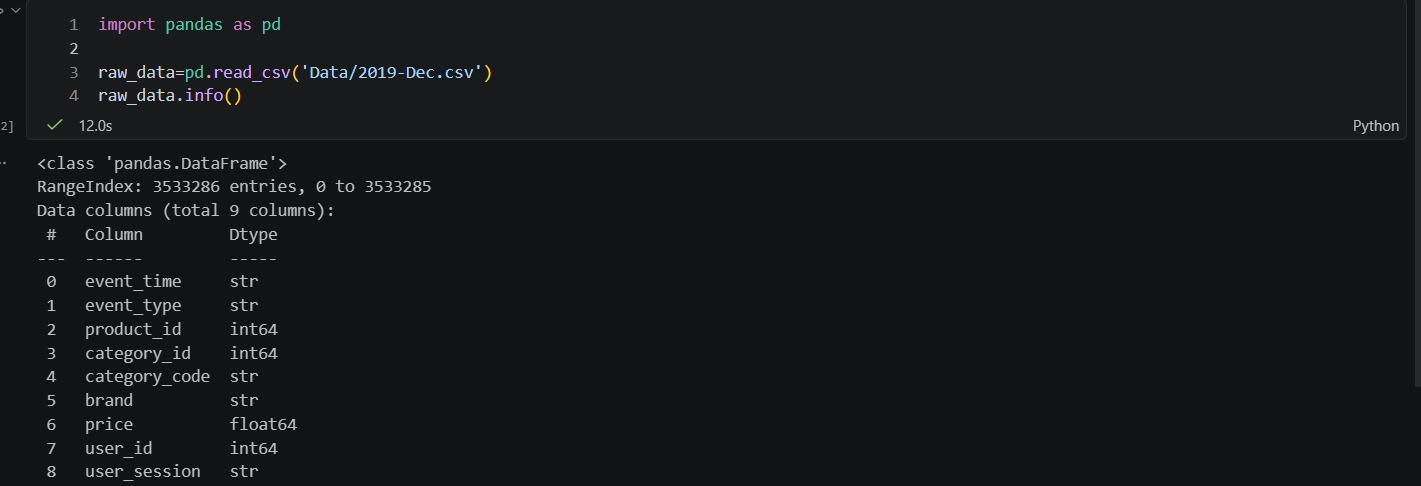
\includegraphics[width=0.8\linewidth]{IMG/Datavalid1.png}
    \caption{Kiểm tra kiểu dữ liệu bằng Python}
\end{figure}

\subsection{Kiểm tra và Đánh giá chất lượng dữ liệu (Data Quality Checks)}
Trước khi trích xuất đặc trưng, dữ liệu thô được kiểm tra toàn diện để phát hiện các điểm bất thường.
\begin{itemize}[itemsep=4pt, leftmargin=*]
    \item \textbf{Kiểm tra kiểu dữ liệu (Data Types):} Cột \texttt{event\_time} ban đầu được hệ thống đọc dưới dạng chuỗi văn bản (Object). Cần phải chuyển đổi sang định dạng \texttt{Datetime} để phục vụ cho việc tính toán thời lượng lướt web.
    \item \textbf{Kiểm tra Dữ liệu thiếu (Missing Values):} Các trường định danh giao dịch (như \texttt{user\_session}, \texttt{event\_type}, \texttt{price}) có tỷ lệ điền đầy 100\%. Tuy nhiên, cột \texttt{brand} (thương hiệu) bị khuyết thiếu khoảng 42\% và \texttt{category\_code} bị khuyết hơn 98\% nên ta có thể xóa cột \texttt{category\_code}. Điều này phản ánh thực tế nghiệp vụ: rất nhiều sản phẩm giá rẻ, không có thương hiệu cụ thể được đăng bán trên sàn.
\begin{figure}[H]
    \centering
    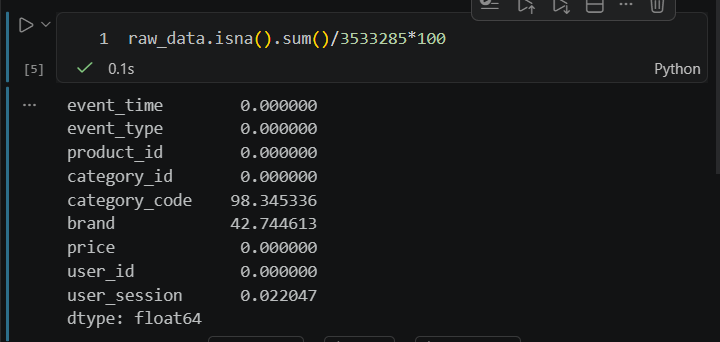
\includegraphics[width=0.8\linewidth]{IMG/NullCheck.png}
    \caption{Kiểm tra null bằng Python}
\end{figure}
    \item \textbf{Kiểm tra Trùng lặp (Duplication):} Trong dữ liệu dạng Log, việc người dùng click đúp (double-click) chuột do lỗi mạng hoặc độ trễ giao diện dẫn đến các bản ghi giống hệt nhau đến từng mili-giây. Dữ liệu ghi nhận khoảng 5.2\% các dòng bị trùng lặp hoàn toàn.
 \begin{figure}[H]
    \centering
     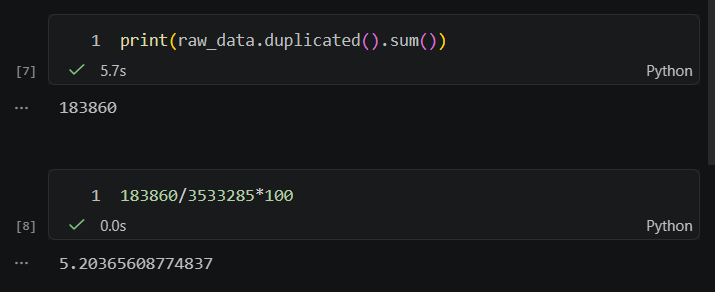
\includegraphics[width=0.8\linewidth]{IMG/DupCheck.png}
       \caption{Kiểm tra trùng lặp bằng Python}
 \end{figure}
    \item     \textbf{Kiểm tra Ngoại lệ (Outliers):} Thống kê mô tả cột \texttt{price} cho thấy xuất hiện một số giá trị âm ($<0$) do lỗi hệ thống backend, và một số sản phẩm có giá cao bất thường (lên tới hàng ngàn USD trong một cửa hàng mỹ phẩm), gây nhiễu cho mô hình.
 \begin{figure}[H]
    \centering
     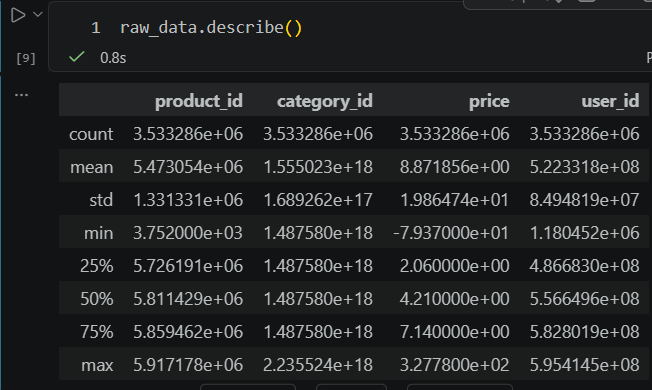
\includegraphics[width=0.8\linewidth]{IMG/Describe.png}
    \caption{Kiểm tra thống kê dữ liệu}
 \end{figure}
\end{itemize}

\subsection{Xử lý dữ liệu và Trích xuất đặc trưng (Data Preprocessing \& Feature Engineering)}
Quy trình xử lý dữ liệu được chia làm 2 giai đoạn: (1) Làm sạch dữ liệu thô và (2) Chuyển đổi định dạng từ dạng dòng (Row-based) sang định dạng phiên (Session-based).

\subsubsection*{Giai đoạn 1: Làm sạch dữ liệu thô (Data Cleaning)}
\begin{itemize}[itemsep=4pt, leftmargin=*]
    \item \textbf{Xử lý trùng lặp và ngoại lệ:} Tiến hành loại bỏ hoàn toàn các dòng trùng lặp (Drop duplicates). Các bản ghi có \texttt{price $\le$ 0} bị loại bỏ vì không mang ý nghĩa kinh doanh. Các mặt hàng có giá lớn hơn phân vị thứ 99 (99th percentile) được giới hạn lại (Winsorization) để giảm tác động của nhiễu.
    \begin{figure}[H]
    \centering
    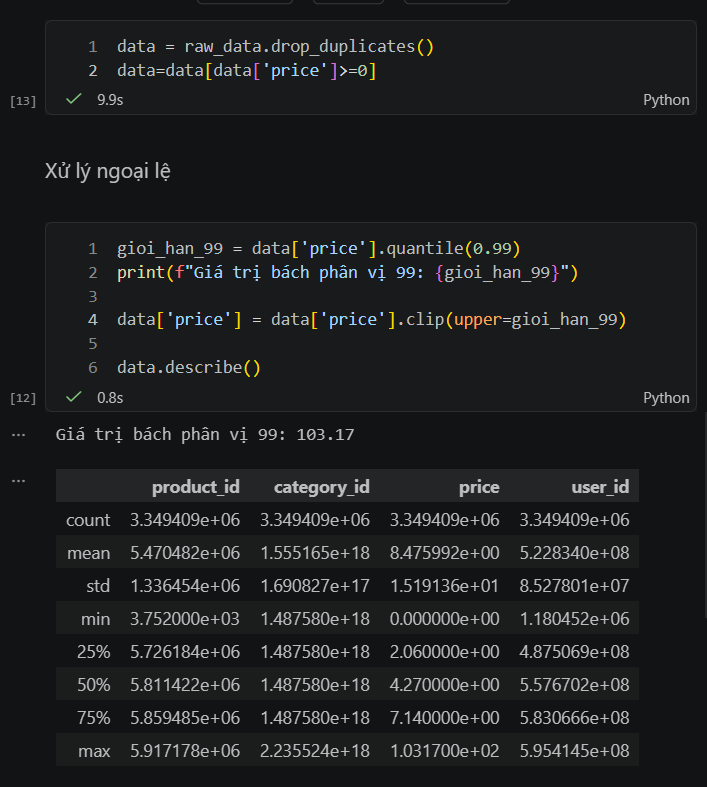
\includegraphics[width=0.8\linewidth]{IMG/ETL1.png}
    \caption{Làm sạch dữ liệu thô}
\end{figure}
    \item \textbf{Xử lý dữ liệu thiếu:} Thay vì xóa bỏ các dòng thiếu \texttt{brand} (sẽ làm mất đi 42\% lượng truy cập), các giá trị \texttt{Null} được điền bằng chuỗi \textit{"Unknown"}. Việc một sản phẩm "Không có thương hiệu" bản chất cũng là một đặc trưng hành vi đáng giá để mô hình học tập. Bên
    cạnh đó ta loại bỏ các cột không đóng góp cho quá trình dự đoán như \texttt{category\_code}, \texttt{User\_id}. Sau đó ta loại bỏ các dòng có \texttt{user\_session} bị null đi (chiếm khoảng 2.2\%)
    \begin{figure}[H]
        \centering
        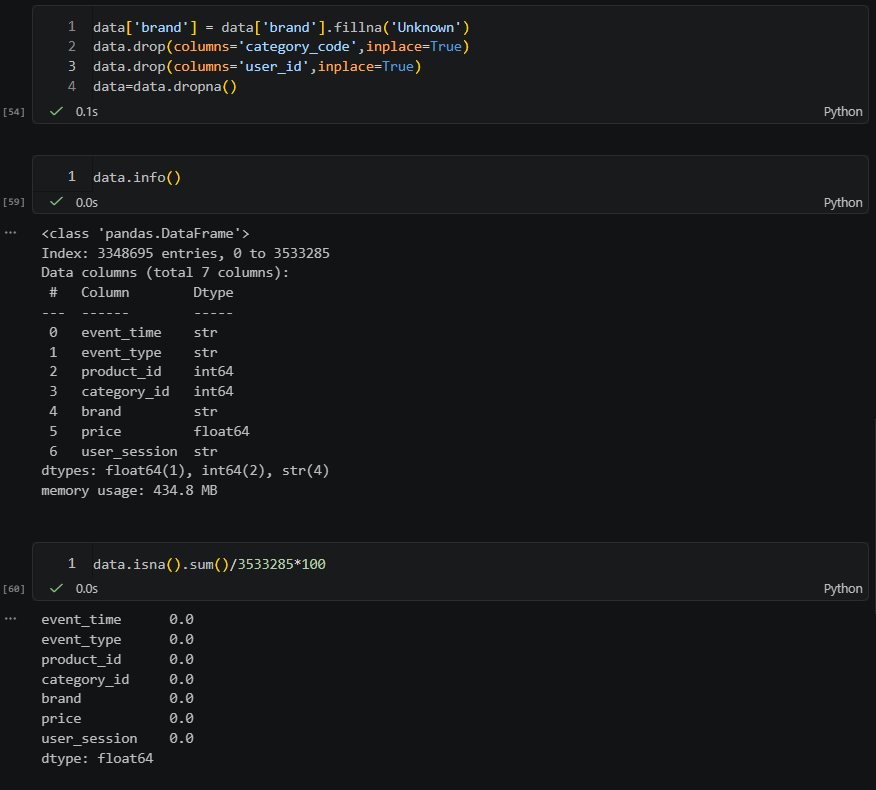
\includegraphics[width=0.8\linewidth]{IMG/ETL2.png}
        \caption{Xử lý khuyết dữ liệu và cột không đóng góp}
    \end{figure}
\end{itemize}

\subsubsection*{Giai đoạn 2: Trích xuất đặc trưng theo Phiên (Sessionization)}
Thuật toán Học máy không thể dự đoán dựa trên từng cú click chuột rời rạc. Dữ liệu được tái cấu trúc (Groupby) theo từng \texttt{user\_session}. Đây là bước quan trọng nhất của đồ án, tuân thủ nguyên tắc ngăn chặn "Rò rỉ dữ liệu" (Data Leakage):
\begin{enumerate}[itemsep=4pt, leftmargin=*]
    \item \textbf{Thiết lập Biến mục tiêu (Target Variable):} Một phiên truy cập được gán nhãn $Y = 1$ (Có mua hàng) nếu trong phiên đó tồn tại ít nhất một sự kiện \texttt{purchase}. Ngược lại gán nhãn $Y = 0$.
    \item \textbf{Tách biệt dữ liệu (Ngăn chặn Leakage):} Toàn bộ các sự kiện \texttt{purchase} được gỡ bỏ khỏi tập huấn luyện. Mô hình chỉ được phép "nhìn" vào lịch sử \texttt{view}, \texttt{cart} để dự đoán.
    \item \textbf{Tổng hợp đặc trưng (Aggregation):} Biến đổi dữ liệu thành các biến định lượng mới:
    \begin{itemize}
        \item \textit{Đặc trưng Hành vi:} \texttt{total\_views} (tổng số lần xem), \texttt{total\_carts} (tổng số lần thêm giỏ), \texttt{session\_duration} (thời lượng phiên tính bằng giây).
        \item \textit{Đặc trưng Tiền tệ:} \texttt{avg\_price}, \texttt{max\_price} (mức giá trung bình khách quan tâm).
        \item \textit{Đặc trưng Đa dạng:} \texttt{unique\_products}, \texttt{unique\_brands}(số lượng các mặt hàng khác nhau đã xem).
    \end{itemize}
    \begin{figure}[H]
    \centering
    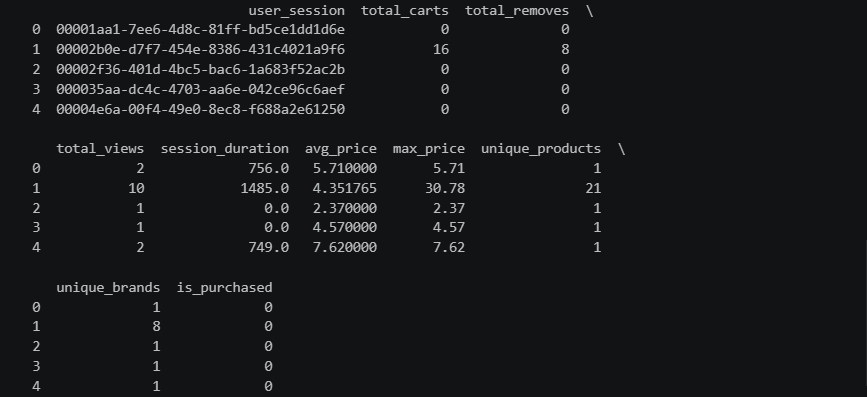
\includegraphics[width=0.8\linewidth]{IMG/ETL3.png}
    \caption{Dữ liệu sau khi tổng hợp đặc trưng}
\end{figure}
    \item \textbf{Chuẩn hóa dữ liệu: } Ta sẽ chuẩn hóa dữ liệu khi sử dụng các mô hình cần chuẩn hóa trước khi dùng.
\end{enumerate}


\section{Khám phá dữ liệu}
Sau quá trình trích xuất đặc trưng (Feature Engineering), việc Phân tích dữ liệu khám phá (EDA) được thực hiện nhằm kiểm tra dữ liệu đã thích hợp để xây dựng mô hình chưa.
\subsection{Phân bố dữ liệu của nhãn}
Ta sẽ vẽ đồ thị thể hiện sô lượng hai nhãn mà ta cần phân:
\begin{figure}[H]
    \centering
    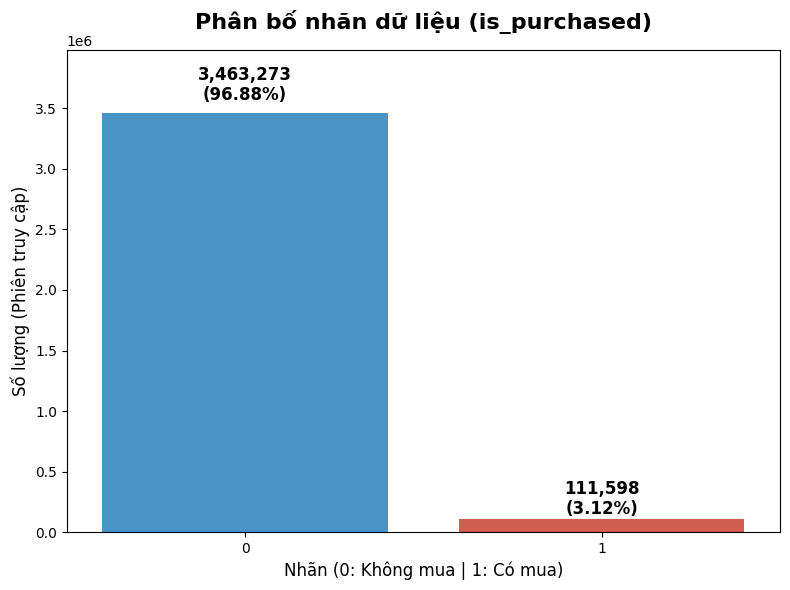
\includegraphics[width=0.8\linewidth]{IMG/phanbonhan.png}
    \caption{Phân bố hai nhãn}
\end{figure}
\textbf{Kết luận}: Từ đây ta thấy được 2 nhãn đang mất cân bằng nghiêm trọng sẽ ảnh hưởng lớn đến mô hình sau này.
\subsection{Phân bố dữ liệu các đặc trưng}
Ta sẽ vẽ đồ thị thể hiện mật độ các giá trị nằm trong mức phân vị thứ 98 của từng biến với hai lớp để so sánh:
\begin{figure}[H]
    \centering
    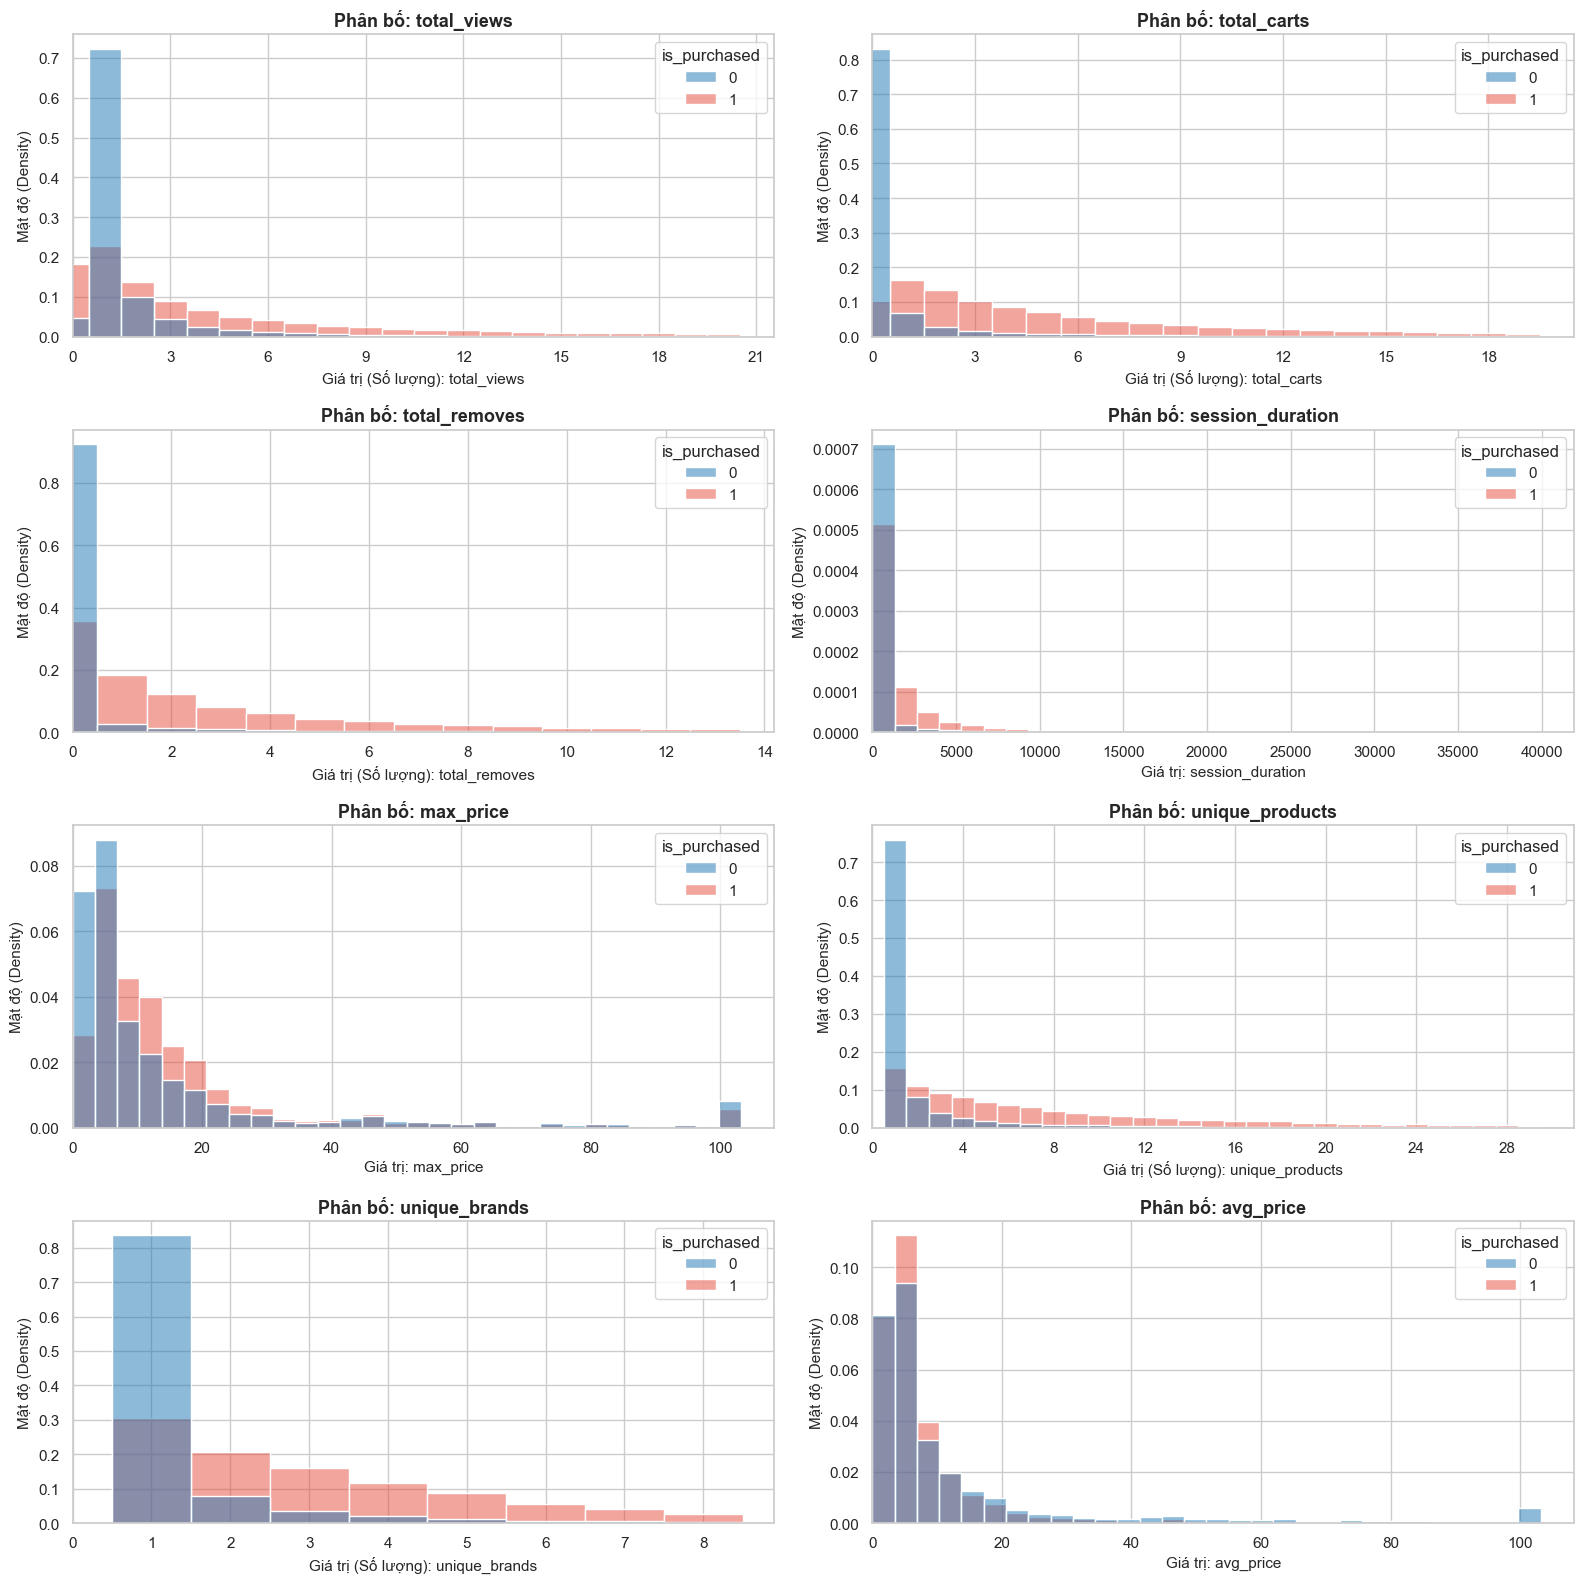
\includegraphics[width=1.2\linewidth]{IMG/feature_distributions.png}
    \caption{Biểu đồ phân bố các biến trong dữ liệu của mô hình}
\end{figure}

Từ biểu đồ này ta thấy được những Insight sau:
\begin{itemize}[itemsep=6pt, leftmargin=*]
    \item \textbf{Insight 1: Đặc điểm của nhóm "Bounce" (Khách hàng thoát trang nhanh)} 
    Quan sát tại biểu đồ \texttt{total\_views} và \texttt{unique\_products}, phân phối của Lớp 0 (Không mua) tạo thành một cột cao đột biến (Spike) ngay tại giá trị bằng 1. Đi kèm với đó, \texttt{session\_duration} của nhóm này cũng tập trung dày đặc ở sát mốc 0 giây. Điều này phác họa chân dung của tệp khách hàng "Click dạo" hoặc "Vào nhầm link": Họ nhấp vào xem đúng một sản phẩm duy nhất và lập tức thoát trang mà không có bất kỳ tương tác nào khác.
    
    \item \textbf{Insight 2: "Thêm vào giỏ" và "Xóa khỏi giỏ" đều là tín hiệu tích cực}
    Biểu đồ \texttt{total\_carts} cho thấy sự phân tách tuyệt đối: Nhóm mua hàng (Lớp 1) chiếm ưu thế hoàn toàn từ giá trị $\ge 1$. Đáng chú ý hơn, tại biểu đồ \texttt{total\_removes}, phân phối của nhóm chốt đơn cũng trải dài về phía bên phải. Về mặt logic kinh doanh, điều này chứng minh rằng thao tác "Xóa sản phẩm khỏi giỏ hàng" không phải là một tín hiệu tiêu cực. Ngược lại, nó thể hiện sự cân nhắc, so sánh và chọn lọc kỹ lưỡng (Active Shopping) của những khách hàng thực sự có ý định mua sắm nghiêm túc.

    \item \textbf{Insight 3: Quy trình "Window Shopping" (So sánh sản phẩm)}
    Biểu đồ \texttt{unique\_products} của nhóm mua hàng có giá trị nằm phần lớn ở khoảng 2 đến 6 sản phẩm. Khách hàng hiếm khi mua ngay sản phẩm đầu tiên họ nhìn thấy. Họ có xu hướng xem nhiều mặt hàng khác nhau để so sánh trước khi đưa ra quyết định cuối cùng.
    
    \item \textbf{Insight 4: Mức giá không quyết định "Ý định mua" (The Price Paradox)}
    Biểu đồ \texttt{avg\_price} là trường hợp đặc biệt nhất khi phân phối của hai lớp 0 và 1 \textbf{gần như chồng khít lên nhau}. Cả hai nhóm đều tập trung xem các sản phẩm ở phân khúc giá thấp và giảm dần ở phân khúc giá cao. Điều này mang lại một phát hiện kinh doanh giá trị: \textit{Giá tiền của sản phẩm không phải là yếu tố phân loại việc khách có chốt đơn trong phiên đó hay không}. Ý định mua hàng được quyết định bởi \textbf{mức độ tương tác sâu} (số lượt xem, thời gian trên trang) chứ không phải bởi giá trị tuyệt đối của món hàng.
\end{itemize}

\subsection{Mối tương quan giữa các đặc trưng}
Sau khi phân tích phân bố của dữ liệu ta đến với việc phân tích tương quan giữa các biến với nhau:
\begin{figure}[H]
    \centering
    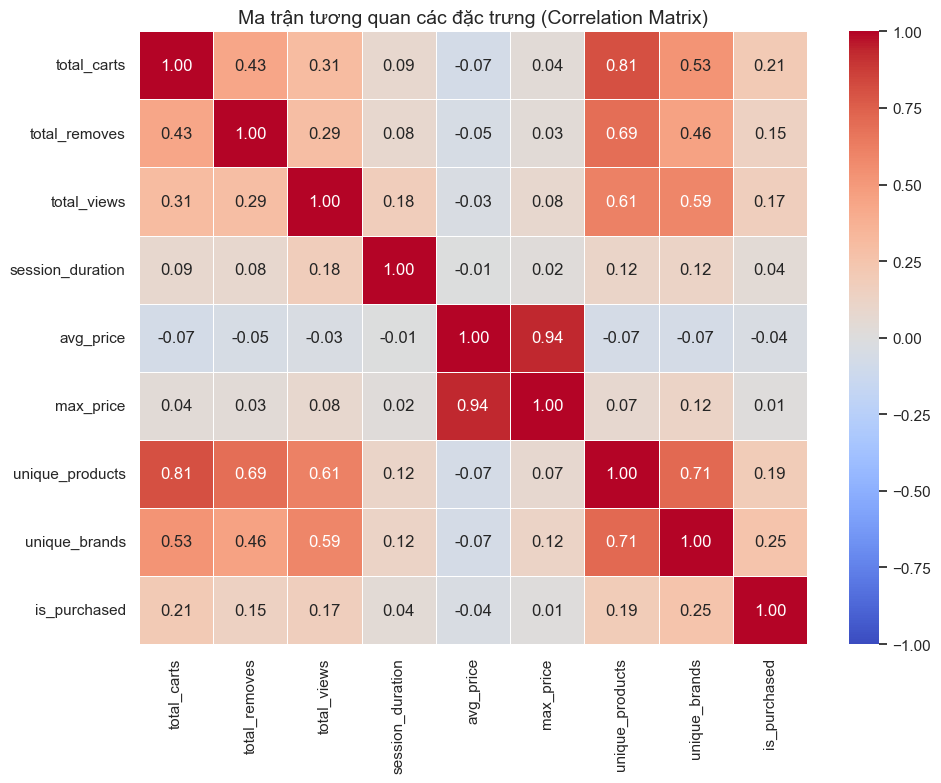
\includegraphics[width=\linewidth]{IMG/Corr.png}
    \caption{Hệ số tương quan giữa các biến}
\end{figure}

Từ biểu đồ này ta thấy được những Insight sau:
\begin{itemize}[itemsep=6pt, leftmargin=*]
  \item \textbf{Insight 1: Hành vi "Thao tác giỏ hàng" là tín hiệu chốt đơn mạnh nhất.} 
    Đối chiếu với biến mục tiêu \texttt{is\_purchased} (hàng dưới cùng), hai biến \texttt{total\_carts} (Thêm giỏ) và \texttt{total\_removes} (Xóa khỏi giỏ) có hệ số tương quan dương cao nhất, cùng đạt mức $0.34$. Trong khi đó, \texttt{total\_views} (Số lượt xem) chỉ đạt $0.12$. Điều này chứng minh bằng toán học rằng: Việc khách hàng xem nhiều sản phẩm không đảm bảo họ sẽ mua hàng (hành vi lướt dạo). Chỉ khi họ bắt đầu có thao tác vật lý với giỏ hàng (cả thêm và xóa), ý định mua sắm mới được xác lập rõ ràng.
    
    \item \textbf{Insight 2: Mức giá hoàn toàn độc lập với Tỷ lệ chuyển đổi.}
    Biến \texttt{avg\_price} (Mức giá trung bình) có hệ số tương quan vô cùng yếu với biến mục tiêu ($-0.02$), gần như xấp xỉ $0$. Hơn thế nữa, nó cũng không tương quan với bất kỳ hành vi lướt web nào khác (tương quan với \texttt{session\_duration} là $-0.02$, với \texttt{total\_views} là $0.06$) Tương tự với \texttt{max\_price}. Phát hiện này tái khẳng định \textit{Nghịch lý Giá cả}: Khách hàng mua đồ đắt hay đồ rẻ đều có tỷ lệ chốt đơn và thời gian lướt web tương đồng nhau. Khách hàng không từ bỏ giỏ hàng chỉ vì món đồ đó đắt, mà vì các yếu tố khác (phí ship, chưa tin tưởng, UI/UX kém...).
    
    \item \textbf{Insight 3: Cụm hành vi "Đa cộng tuyến" (Behavioral Clustering).}
    Kiểm tra tương quan giữa các biến độc lập, hệ thống ghi nhận một cụm biến có tương quan thuận cực kỳ mạnh: \texttt{session\_duration} và \texttt{unique\_products} đạt mức $0.84$; \texttt{session\_duration} và \texttt{total\_views} đạt $0.69$. Về mặt logic, điều này rất hợp lý: Khách hàng ở lại trang càng lâu (duration) thì họ càng xem nhiều lượt (views) và tiếp cận nhiều sản phẩm khác nhau (unique).
\end{itemize}

\textbf{Kết luận: }Ta có thể bỏ cột \texttt{avg\_price} để làm tăng tốc độ train mô hình và loại bỏ nhiễu. Với các mô hình tuyến tính 
ta cần phải lựa chọn bỏ bớt một biến để tránh sai số do hiện tượng Đa cộng tuyến.
\section{Huấn luyện mô hình}
\subsection*{Mục tiêu mô hình}
Mục tiêu cốt lõi của bước này là xây dựng một hệ thống phân loại nhị phân (Binary Classification) có khả năng dự đoán chính xác việc một phiên truy cập (Session) có dẫn đến hành vi thanh toán (Purchase) hay không. Do tính chất đặc thù của dữ liệu Thương mại điện tử, việc đánh giá mô hình sẽ không phụ thuộc vào Độ chính xác tổng thể (Accuracy), mà được định hướng tối ưu hóa dựa trên \textbf{F1-Score} (giữ sự cân bằng) và \textbf{Độ phủ (Recall)} nhằm đảm bảo doanh nghiệp không bỏ lọt các khách hàng tiềm năng, phục vụ trực tiếp cho các chiến dịch Remarketing thời gian thực.

\subsection*{Xử lý đặc trưng gây nhiễu (Feature Selection)}
Qua quá trình phân tích Khám phá dữ liệu (EDA) và Ma trận tương quan, ta nhận thấy hai đặc trưng về giá trị tiền tệ là \texttt{avg\_price} và \texttt{max\_price} gần như không có tương quan tuyến tính với biến mục tiêu (hệ số xấp xỉ 0). Sự tồn tại của các biến này không đóng góp vào năng lực phân loại mà còn có nguy cơ tạo ra nhiễu (Noise). Do đó, ta tiến hành loại bỏ hai cột này khi làm việc với các mô hình phân loại tuyến tính nhằm giảm số chiều dữ liệu và tăng tính ổn định cho thuật toán.

\subsection{Xử lý mất cân bằng dữ liệu (Class Imbalance Handling)}
Để xử lý hiện tượng mất cân bằng lớp nghiêm trọng trong tập dữ liệu này, thay vì sử dụng kỹ thuật Undersampling truyền thống (vốn gây thất thoát lượng lớn thông tin của lớp đa số), ta sẽ áp dụng chiến lược \textbf{Ensemble-based Undersampling}. 

Cụ thể, bộ dữ liệu gốc sẽ được chia thành $n$ bộ dữ liệu con (Subsets). Trong mỗi bộ con, toàn bộ các bản ghi thuộc lớp thiểu số (Nhãn 1 - Có mua hàng) được giữ nguyên, kết hợp với một lượng bản ghi thuộc lớp đa số (Nhãn 0 - Không mua) được lấy mẫu ngẫu nhiên sao cho tỷ lệ thích hợp. Phương pháp này không chỉ đảm bảo từng mô hình con được học trên một không gian cân bằng hoàn hảo, mà việc tổng hợp kết quả (Voting/Averaging) từ $n$ mô hình còn giúp tận dụng triệt để toàn bộ thông tin của lớp 0 ban đầu, từ đó giảm thiểu phương sai (Variance) và chống quá khớp (Overfitting).

Bên cạnh đó ta sẽ điều chỉnh \textbf{ngưỡng quyết định} thích hợp cho mô hình để gia tăng độ chính xác.
\subsection{Xây dựng mô hình (Model Building)}
Ta sẽ xây dựng mô hình cơ bản là Cây quyết định (Decision Tree) và \textit{tiếp tục phát triển mở rộng lên các thuật toán Học máy kết hợp (Ensemble Learning) mạnh mẽ hơn}. Quy trình huấn luyện được cấu trúc theo các cấp độ sau:

\begin{itemize}[itemsep=4pt, leftmargin=*]
    \item \textbf{Mô hình cơ sở (Baseline Models):} Bắt đầu với \textbf{Hồi quy Logistic (Logistic Regression)} để kiểm tra khả năng phân tách tuyến tính của dữ liệu, và \textbf{Cây quyết định (Decision Tree)} để thiết lập bộ luật cơ bản (If-Else Rules), giúp đánh giá mô hình.
    
    \item \textbf{Mô hình kết hợp (Ensemble Models):} Áp dụng \textbf{Random Forest} — một tập hợp của nhiều cây quyết định hoạt động độc lập, kết hợp cùng chiến lược lấy mẫu chia nhỏ tập dữ liệu (như đã đề cập ở phần Xử lý mất cân bằng) nhằm cải thiện độ chuẩn xác (Precision).
    
    \item \textbf{Mô hình Tăng cường độ dốc (Gradient Boosting Trees):} Sử dụng các thuật toán tối tân nhất đối với dữ liệu dạng bảng như \textbf{XGBoost} và \textbf{LightGBM}. Bản chất học tập tuần tự (cây sau sửa lỗi cho cây trước) kết hợp cùng hàm mục tiêu tối ưu hóa đặc biệt sẽ giúp hệ thống vắt kiệt tối đa sức mạnh của tập đặc trưng hành vi, đẩy F1-Score lên mức cao nhất có thể.
\end{itemize}
\section{Kết quả và đánh giá}
\subsection{Kết quả Baseline Model}
Ta chọn mô hình cơ sở là mô hình \textbf{Hồi quy Logistic (Logistic Regression)}. Sau khi tìm được mô hình ta thử với từng \textbf{ngưỡng quyết định} thì với ngưỡng quyết định là 0.73 thì có chỉ số F1 cao nhất. \\


\vspace{0.5cm}

\begin{table}[H]
\centering
\begin{tabular}{lcccc}
\toprule
 & \textbf{precision} & \textbf{recall} & \textbf{f1-score} & \textbf{support} \\
\midrule
\textbf{0} & 0.98 & 0.95 & 0.97 & 692655 \\
\textbf{1} & 0.24 & 0.49 & 0.32 & 22320 \\
\midrule
\textbf{accuracy} & & & 0.94 & 714975 \\
\textbf{macro avg} & 0.61 & 0.72 & 0.64 & 714975 \\
\textbf{weighted avg} & 0.96 & 0.94 & 0.95 & 714975 \\
\bottomrule
\end{tabular}
\caption{Các Metric của mô hình Hồi quy Logistic (Logistic Regression)}
\end{table}

\vspace{0.5cm}

\subsection{Kết quả trước khi xử lý mất cân bằng}
Mô hình ta chọn sẽ là mô hình \textbf{Cây quyết định} do đặc thù của dữ liệu. Sau khi phân nhãn và chọn được ngưỡng tối ưu là 0.88 ta thu được các metric như sau:
\begin{table}[H]
\centering
\begin{tabular}{lcccc}
\toprule
 & \textbf{precision} & \textbf{recall} & \textbf{f1-score} & \textbf{support} \\
\midrule
\textbf{0} & 0.98 & 0.95 & 0.97 & 692655 \\
\textbf{1} & 0.27 & 0.52 & 0.35 & 22320 \\
\midrule
\textbf{accuracy} & & & 0.94 & 714975 \\
\textbf{macro avg} & 0.63 & 0.74 & 0.66 & 714975 \\
\textbf{weighted avg} & 0.96 & 0.94 & 0.95 & 714975 \\
\bottomrule
\end{tabular}
\caption{Các Metric của mô hình cây quyết định}
\end{table}
\begin{figure}[H]
    \centering
    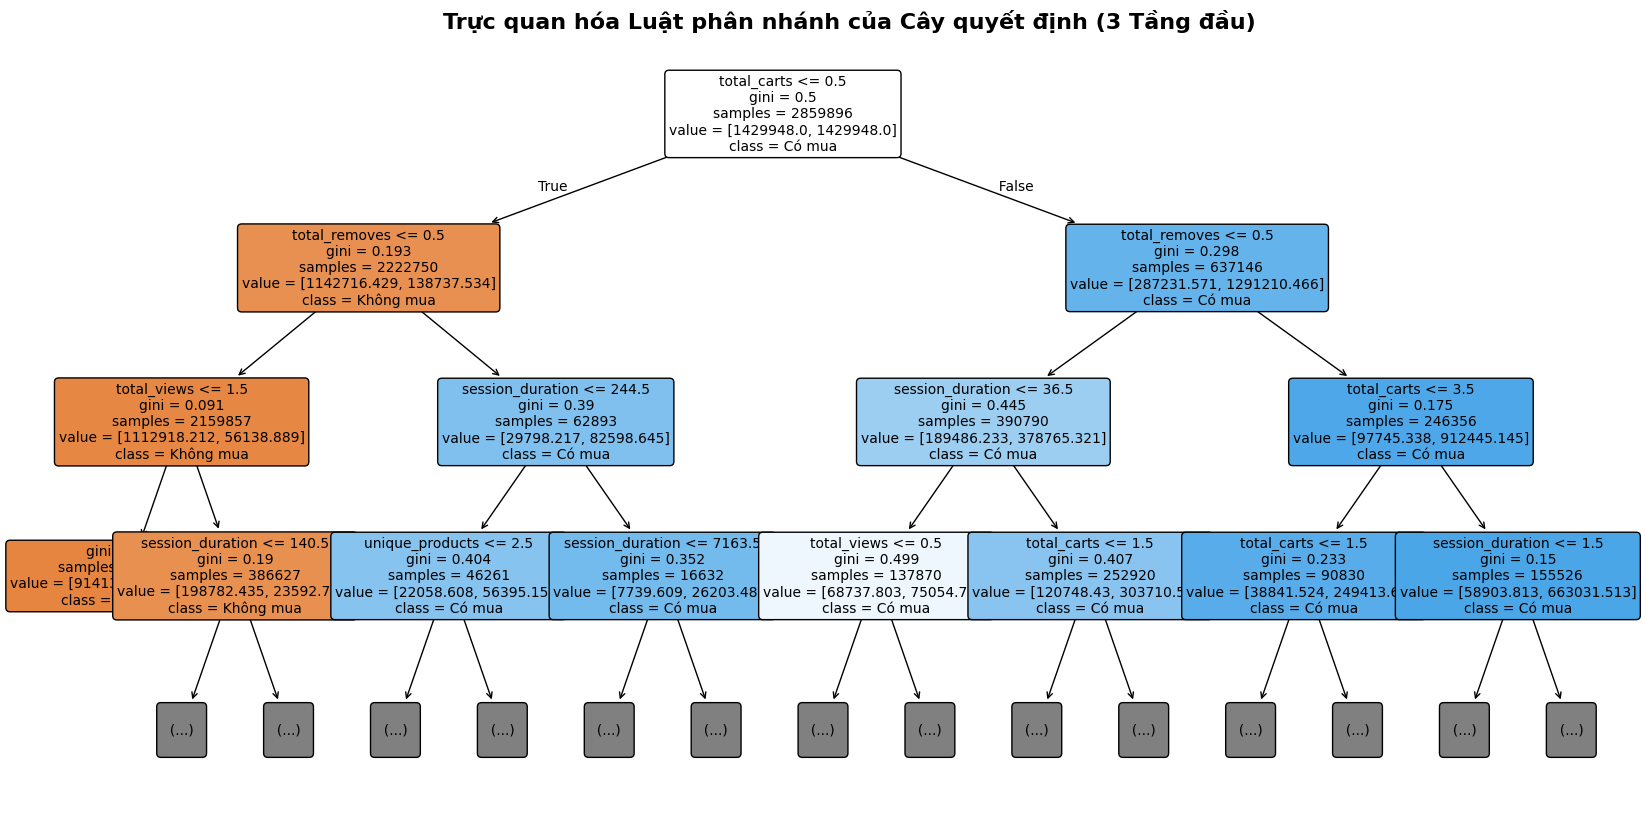
\includegraphics[width=0.8\linewidth]{IMG/cayquyetdinh.png}
    \caption{3 tầng đầu cây quyết định}
\end{figure}
Bên cạnh đó ta còn sử dụng mô hình \textbf{lightGBM} nhằm tăng Recall và F1. Sau khi xây dựng mô hình và chọn ngưỡng ta thu được các metric như sau:
\begin{table}[H]
\centering
\begin{tabular}{lcccc}
\toprule
 & \textbf{precision} & \textbf{recall} & \textbf{f1-score} & \textbf{support} \\
\midrule
\textbf{0} & 0.98 & 0.95 & 0.97 & 692655 \\
\textbf{1} & 0.29 & 0.55 & 0.37 & 22320 \\
\midrule
\textbf{accuracy} & & & 0.94 & 714975 \\
\textbf{macro avg} & 0.64 & 0.75 & 0.67 & 714975 \\
\textbf{weighted avg} & 0.96 & 0.94 & 0.95 & 714975 \\
\bottomrule
\end{tabular}
\caption{Các Metric của mô hình lightGBM}
\end{table}
\subsection{Kết quả sau khi xử lý mất cân bằng}
Sau khi xây dựng mô hình Esemble bằng cách tạo các mô hình cây quyết định con và 
phân phối dữ liệu thành 11 phần bằng nhau, có phần nhãn=1 giống nhau nhưng phần nhãn bằng 0 khác nhau lúc này 
dữ liệu của các mô hình con tỷ lệ nhãn 0 / nhãn 1 = 3, giảm rất nhiều so với dữ liệu ban đầu nhưng không làm mất dữ liệu.

Sau khi xây dựng mô hình và chọn ngưỡng 0.88
\begin{table}[H]
\centering
\begin{tabular}{lcccc}
\toprule
 & \textbf{precision} & \textbf{recall} & \textbf{f1-score} & \textbf{support} \\
\midrule
\textbf{0} & 0.98 & 0.96 & 0.97 & 692655 \\
\textbf{1} & 0.27 & 0.51 & 0.36 & 22320 \\
\midrule
\textbf{accuracy} & & & 0.94 & 714975 \\
\textbf{macro avg} & 0.63 & 0.74 & 0.66 & 714975 \\
\textbf{weighted avg} & 0.96 & 0.94 & 0.95 & 714975 \\
\bottomrule
\end{tabular}
\caption{Metric của mô hình Ensemble cây quyết định (Random Forest + Bagging)}
\end{table}

Làm tương tự với mô hình \textbf{lightGBM} và ngưỡng quyết định ta thu được các metric như sau:
\begin{table}[h]
\centering
\begin{tabular}{lcccc}
\toprule
 & \textbf{precision} & \textbf{recall} & \textbf{f1-score} & \textbf{support} \\
\midrule
\textbf{0} & 0.99 & 0.95 & 0.97 & 692655 \\
\textbf{1} & 0.27 & 0.61 & 0.37 & 22320 \\
\midrule
\textbf{accuracy} & & & 0.94 & 714975 \\
\textbf{macro avg} & 0.63 & 0.78 & 0.67 & 714975 \\
\textbf{weighted avg} & 0.96 & 0.94 & 0.95 & 714975 \\
\bottomrule
\end{tabular}
\caption{Mô hình lightGBM sau khi xử lý mất cân bằng}
\end{table}
\subsection{Đánh giá}
\begin{itemize}[itemsep=6pt, leftmargin=*]
    \item \textbf{Sức mạnh nội tại của thuật toán (Algorithm Intrinsic Power):} 
    Ngay từ giai đoạn chưa xử lý mất cân bằng, mô hình \textbf{LightGBM} đã cho thấy sự vượt trội hoàn toàn so với mô hình Cây quyết định đơn lẻ (Decision Tree). Điểm F1-Score của LightGBM đạt $0.37$ so với $0.35$ của Cây quyết định, đồng thời cải thiện cả Độ phủ (Recall từ $0.52$ lên $0.55$) và Độ chuẩn xác (Precision từ $0.27$ lên $0.29$). Điều này chứng minh cơ chế Tăng cường độ dốc (Gradient Boosting) có khả năng tối ưu hóa hàm mất mát trên dữ liệu phi tuyến tốt hơn nhiều so với một cây quyết định độc lập.

    \item \textbf{Hiệu năng của Kiến trúc Ensemble Phân mảnh (Chunking Ensemble):} 
    Sự thành công lớn nhất của nghiên cứu nằm ở việc áp dụng chiến lược chia nhỏ tập đa số (Lớp 0) thành 11 phần để kết hợp với tập thiểu số (Lớp 1). Khi so sánh giữa mô hình LightGBM trước và sau khi áp dụng kiến trúc Ensemble, ta quan sát thấy \textbf{Hiện tượng đánh đổi (Precision-Recall Trade-off)} diễn ra vô cùng rõ nét nhưng mang lại giá trị cao:
    \begin{itemize}
        \item Độ chuẩn xác (Precision) giảm nhẹ $2\%$ (từ $0.29$ xuống $0.27$).
        \item Tuy nhiên, Độ phủ (Recall) lại có bước nhảy vọt \textbf{tăng $6\%$} (từ $0.55$ lên $0.61$), giữ cho điểm F1-Score ổn định ở mức tối đa là $0.37$.
    \end{itemize}

    \item \textbf{Đánh giá dưới góc độ Kinh doanh (Business Perspective):} 
    Với tổng số $22.320$ khách hàng thực sự chốt đơn trong tập kiểm thử, mức tăng $6\%$ Recall đồng nghĩa với việc kiến trúc Ensemble LightGBM đã nhận diện thành công thêm khoảng \textbf{$1.339$ khách hàng tiềm năng} có nguy cơ bị bỏ sót bởi mô hình LightGBM nguyên thủy. Trong nghiệp vụ Thương mại điện tử, chi phí để tiếp cận khách hàng (như gửi Email tự động, Push Notification) là nhỏ so với doanh thu thu được. Việc hy sinh $2\%$ Precision để mở rộng tệp khách hàng bắt trúng mang lại \textbf{Lợi nhuận ròng (Net Profit) vượt trội} so với các mô hình còn lại.
\end{itemize}

\textbf{Kết luận:} Dựa trên khả năng tối đa hóa độ phủ khách hàng tiềm năng, duy trì sự ổn định của phương sai nhờ cơ chế Bỏ phiếu mềm (Soft Voting) từ 11 mô hình con, \textbf{Ensemble LightGBM} kết hợp thuật toán tự động tinh chỉnh ngưỡng được quyết định lựa chọn làm Mô hình triển khai chính thức (Production Model) cho hệ thống dự đoán hành vi Thương mại điện tử.
\section{Khuyến nghị ra quyết định}
\subsection{Khuyến nghị}
Dựa trên kết quả triển khai mô hình Ensemble LightGBM và các phát hiện từ quá trình Khám phá dữ liệu (EDA), hệ thống không chỉ dừng lại ở việc dự đoán chính xác ý định mua hàng mà còn mở ra cơ hội tái cấu trúc toàn diện chiến lược vận hành của doanh nghiệp Thương mại điện tử. Dưới đây là 4 khuyến nghị chiến lược nhằm chuyển hóa sức mạnh của Trí tuệ nhân tạo (AI) thành Lợi nhuận ròng (Net Profit):

\subsection*{1. Chuyển dịch từ Marketing đại trà sang Marketing mục tiêu (Targeted Retargeting)}
\begin{itemize}[itemsep=4pt, leftmargin=*]
    \item \textbf{Cơ sở dữ liệu:} Mô hình đề xuất đạt Độ phủ (Recall) $61\%$ và Độ chuẩn xác (Precision) $27\%$.
    \item \textbf{Khuyến nghị:} Doanh nghiệp cần chấm dứt việc chạy quảng cáo bám đuôi (Retargeting Ads trên Facebook, Google) hoặc gửi Email Marketing cho toàn bộ $100\%$ khách hàng truy cập website. Thay vào đó, ngân sách quảng cáo chỉ nên giải ngân vào danh sách khách hàng được mô hình gán nhãn \textbf{1 (Có ý định mua)}. 
    \item \textbf{Lợi ích kinh tế:} Mặc dù Precision là $27\%$, tỷ lệ này đã cao hơn gấp $10$ đến $15$ lần so với tỷ lệ chuyển đổi tự nhiên (Organic Conversion Rate thường ở mức $2\%$). Điều này giúp doanh nghiệp giảm thiểu triệt để Chi phí thu hút khách hàng (CAC - Customer Acquisition Cost) và tăng vọt Lợi tức đầu tư quảng cáo (ROAS).
\end{itemize}

\subsection*{2. Chiến lược phân phối Khuyến mãi thông minh (Smart Vouchering)}
\begin{itemize}[itemsep=4pt, leftmargin=*]
    \item \textbf{Cơ sở dữ liệu:} Phân tích Tương quan chỉ ra mức giá (\texttt{avg\_price}) không ảnh hưởng tới quyết định mua, nhưng các tương tác giỏ hàng (\texttt{total\_carts}, \texttt{total\_removes}) lại là tín hiệu chốt đơn cực kỳ mạnh.
    \item \textbf{Khuyến nghị:} Không phát mã giảm giá (Voucher) một cách mù quáng. Hệ thống CRM cần tích hợp mô hình AI để phân luồng người dùng theo Xác suất dự đoán (Probability Score):
    \begin{itemize}
        \item \textbf{Xác suất $> 90\%$ (Chắc chắn mua):} Khách hàng đã quyết tâm mua. \textbf{Không cấp Voucher} để bảo vệ biên lợi nhuận tuyệt đối.
        \item \textbf{Xác suất từ $70\% - 90\%$ (Đang phân vân):} Khách hàng có thao tác thêm và xóa khỏi giỏ nhiều lần. Hệ thống tự động kích hoạt một \textbf{Pop-up Voucher Freeship có thời hạn 15 phút}. Hiệu ứng tâm lý sợ bỏ lỡ (FOMO) sẽ ép khách hàng chốt đơn ngay lập tức thay vì thoát trang.
        \item \textbf{Xác suất $< 50\%$ (Chỉ lướt dạo):} \textbf{Không cấp Voucher}, thay vào đó hiển thị giao diện gợi ý các bài viết blog làm đẹp hoặc các sản phẩm xu hướng để thu thập Email (Lead Generation).
    \end{itemize}
\end{itemize}

\subsection*{3. Can thiệp Chăm sóc khách hàng theo Thời gian thực (Real-time Intervention)}
\begin{itemize}[itemsep=4pt, leftmargin=*]
    \item \textbf{Khuyến nghị:} Tích hợp mô hình Ensemble trực tiếp vào hệ thống Backend (sử dụng công nghệ truyền phát dữ liệu thời gian thực như Apache Kafka). 
    \item \textbf{Quy trình hành động:} Khi hệ thống ghi nhận một phiên truy cập có Thời lượng (\texttt{session\_duration}) lớn hơn mức trung bình và Xác suất chốt đơn cao, nhưng khách hàng lại dừng lại quá 3 phút ở trang Thanh toán (Checkout), hệ thống sẽ gửi cảnh báo đến bộ phận Chăm sóc khách hàng (CSKH). Nhân viên CSKH sẽ chủ động nhắn tin qua Live-chat: \textit{"Chào bạn, hệ thống ghi nhận bạn đang gặp khó khăn khi thanh toán, mình có thể hỗ trợ bạn không?"}. Sự can thiệp đúng lúc này là "chìa khóa vàng" để cứu vãn các giỏ hàng có giá trị cao bị bỏ rơi do lỗi kỹ thuật hoặc thiếu thông tin.
\end{itemize}

\subsection*{4. Tối ưu hóa Trải nghiệm Người dùng (Dynamic UI/UX)}
\begin{itemize}[itemsep=4pt, leftmargin=*]
    \item \textbf{Cơ sở dữ liệu:} Thuật toán phân định rõ nhóm "Bounce" (Vào xem đúng 1 sản phẩm rồi thoát) và nhóm "Active Shopping" (Xem nhiều, tương tác nhiều).
    \item \textbf{Khuyến nghị:} Giao diện website/ứng dụng cần được cá nhân hóa tự động. Đối với nhóm được dự đoán \textbf{Nhãn 0}, giao diện nên hiển thị dạng "Khám phá" (Discovery Mode) với nhiều hình ảnh bắt mắt để giữ chân họ trên nền tảng. Ngược lại, với nhóm được dự đoán \textbf{Nhãn 1}, giao diện cần tự động ẩn đi các banner quảng cáo rườm rà, đẩy nút \textbf{"Thanh toán ngay"} lên vị trí trung tâm màn hình, rút gọn tối đa số lần nhấp chuột (Click) để quá trình chốt đơn diễn ra mượt mà nhất.
\end{itemize}
\subsection{Đánh giá Rủi ro và Hạn chế của hệ thống (Risks \& Limitations)}

Mặc dù hệ thống Ensemble LightGBM mang lại những định hướng kinh doanh rõ nét, việc áp dụng trí tuệ nhân tạo vào môi trường Thương mại điện tử thực tế luôn đi kèm với những rủi ro và giới hạn nhất định. Nhằm đảm bảo tính an toàn trong vận hành, doanh nghiệp cần lưu ý các vấn đề sau trước khi triển khai (Deployment):

\subsubsection*{1. Hạn chế về mặt Dữ liệu và Mô hình (Technical Limitations)}
\begin{itemize}[itemsep=4pt, leftmargin=*]
    \item \textbf{Giới hạn của dữ liệu theo Phiên (Session-based Constraint):} Mô hình hiện tại phân tích hành vi dựa trên từng \texttt{user\_session} độc lập. Trong thực tế, chu kỳ mua sắm của khách hàng (Customer Journey) có thể kéo dài qua nhiều phiên hoặc vắt chéo qua nhiều thiết bị (Cross-device tracking) — ví dụ: khách hàng xem sản phẩm trên điện thoại nhưng thanh toán trên máy tính. Việc mô hình chưa liên kết được các chuỗi phiên này có thể làm giảm khả năng nhận diện ý định mua sắm dài hạn.
    \item \textbf{Hiện tượng trôi dạt khái niệm (Concept Drift):} Dữ liệu huấn luyện được thu thập trong khoảng thời gian cụ thể (Tháng 10 - Tháng 2). Thói quen mua sắm của người tiêu dùng có tính mùa vụ (Seasonality) rất cao (ví dụ: hành vi mua sắm dịp Black Friday sẽ rất khác so với mùa hè). Nếu không thiết lập cơ chế tự động huấn luyện lại (Retraining Pipeline) định kỳ, hiệu năng của mô hình sẽ bị suy giảm theo thời gian do dữ liệu lỗi thời.
\end{itemize}

\subsubsection*{2. Rủi ro trong Triển khai Kinh doanh (Business Implementation Risks)}
\begin{itemize}[itemsep=4pt, leftmargin=*]
    \item \textbf{Rủi ro thất thoát tài chính từ False Positives (Báo động giả):} Mặc dù mô hình đạt Recall 61\%, chỉ số Độ chuẩn xác (Precision) vẫn dừng ở mức 27\%. Nghĩa là trong 100 khách hàng được dự đoán "Sắp mua", có 73 khách hàng thực chất không mua. Nếu doanh nghiệp sử dụng danh sách này cho các chiến dịch có \textbf{Chi phí biên cao (High Marginal Cost)} — ví dụ như gọi điện Telesales trực tiếp hoặc tặng Voucher giá trị lớn ($>100.000$ VNĐ) — sự nhầm lẫn của mô hình sẽ gây lãng phí ngân sách nghiêm trọng. Khuyến nghị này chỉ an toàn với các chiến dịch chi phí thấp (Email, Push Notification).
    
    \item \textbf{Rủi ro thao túng thuật toán (System Gaming / Voucher Abuse):} Nếu thuật toán tặng Voucher tự động (đã đề cập ở mục trên) hoạt động quá nguyên tắc, một bộ phận khách hàng thông minh có thể "bắt bài" hệ thống. Họ sẽ cố tình thực hiện các thao tác thêm/xóa giỏ hàng và ngâm trang lâu để ép AI phải nhả mã giảm giá. Để phòng tránh, hệ thống cần bổ sung \textit{Cơ chế giới hạn tần suất (Rate Limiting)} và \textit{Phân phối ngẫu nhiên (Randomization)} đối với mỗi \texttt{user\_id}.
    
    \item \textbf{Rủi ro gián đoạn trải nghiệm người dùng (UX Disruption):} Việc can thiệp thời gian thực (Real-time Intervention) như bật Pop-up hay Live-chat nếu diễn ra quá dày đặc sẽ gây phản tác dụng, khiến khách hàng cảm thấy bị làm phiền hoặc mất quyền riêng tư (Privacy Concerns). 
\end{itemize}

\textbf{Giải pháp khắc phục chung:} Trước khi triển khai toàn hệ thống, doanh nghiệp bắt buộc phải thực hiện \textbf{Kiểm thử A/B (A/B Testing)} trên một tệp khách hàng nhỏ (ví dụ $10\%$ lưu lượng truy cập). Chỉ khi kết quả A/B Testing chứng minh được Lợi nhuận ròng (Net Profit) của nhóm dùng AI cao hơn có ý nghĩa thống kê so với nhóm đối chứng (Control Group), mô hình mới được phép triển khai diện rộng (Mass Rollout).
\section{Hạn chế và hướng phát triển}
\subsection{Hạn chế của dữ liệu và mô hình hiện tại (Limitations)}
Mặc dù kiến trúc Ensemble LightGBM đã mang lại những cải thiện đáng kể về năng lực dự báo, nghiên cứu vẫn tồn tại một số giới hạn nhất định về mặt khai thác dữ liệu và bản chất thuật toán:

\begin{itemize}[itemsep=4pt, leftmargin=*]
    \item \textbf{Giới hạn phạm vi phiên truy cập đơn lẻ (Single-session Constraint):} 
    Quá trình trích xuất đặc trưng (Feature Engineering) hiện tại đang gom nhóm (Groupby) dữ liệu theo từng \texttt{user\_session} độc lập. Tuy nhiên, hành vi mua sắm thực tế thường là một hành trình kéo dài (Customer Journey). Một khách hàng có thể lướt xem sản phẩm trên điện thoại vào buổi sáng (Phiên 1), sau đó đăng nhập trên máy tính để thanh toán vào buổi tối (Phiên 2). Việc mô hình đánh giá rời rạc từng phiên đã vô tình làm mất đi sự liên kết thông tin lịch sử của cùng một \texttt{user\_id}.
    
    \item \textbf{Bỏ qua tính tuần tự của chuỗi hành vi (Lack of Sequential Dynamics):} 
    Các đặc trưng được tổng hợp như \texttt{total\_views}, \texttt{total\_carts} chỉ mang tính chất thống kê số đếm (Aggregated Counts) mà không phản ánh được \textit{thứ tự} xảy ra của các sự kiện. Về mặt logic, một phiên truy cập có thứ tự hành vi: \texttt{View $\rightarrow$ View $\rightarrow$ Cart} sẽ có xác suất chốt đơn cao hơn rất nhiều so với chuỗi \texttt{Cart $\rightarrow$ View $\rightarrow$ Remove}. Mô hình dữ liệu dạng bảng (Tabular Models) như LightGBM chưa có khả năng học được luồng thời gian (Time-series) vi mô này.
    
    \item \textbf{Giới hạn trong xử lý thông tin định danh (Categorical \& Textual Limits):}
    Tập dữ liệu chứa nhiều biến mang thông tin danh mục như \texttt{category\_code} hoặc \texttt{brand}. Nghiên cứu hiện tại mới chỉ xử lý ở mức độ cơ bản (Loại bỏ hoặc điền Unknown) do tỷ lệ khuyết thiếu cao. Điều này làm lãng phí một phần tri thức về sở thích thương hiệu (Brand Loyalty) của người dùng.
\end{itemize}

\subsection{Hướng phát triển trong tương lai (Future Work)}
Từ những hạn chế nêu trên, nghiên cứu đề xuất các hướng mở rộng và nâng cấp hệ thống trong tương lai nhằm đưa mô hình tiệm cận với mức độ hoàn hảo của các hệ thống AI công nghiệp:

\begin{itemize}[itemsep=4pt, leftmargin=*]
    \item \textbf{Ứng dụng Học Sâu cho chuỗi thời gian (Deep Learning for Sequential Data):} 
    Thay vì sử dụng phương pháp gom nhóm thống kê truyền thống, hướng phát triển cốt lõi là chuyển đổi bài toán sang dạng Dự đoán chuỗi (Sequence Prediction). Các mạng nơ-ron hồi quy như \textbf{RNN, LSTM (Long Short-Term Memory)} hoặc kiến trúc \textbf{Transformer (Self-Attention Models)} sẽ được áp dụng để đưa trực tiếp chuỗi click chuột theo thứ tự thời gian vào huấn luyện. Kỹ thuật này giúp mô hình "hiểu" được ngữ cảnh của từng thao tác lướt web trước khi khách hàng ra quyết định.
    
    \item \textbf{Kết hợp Hồ sơ Lịch sử Người dùng (User Profiling \& RFM):} 
    Tiến hành liên kết các \texttt{user\_session} thông qua \texttt{user\_id} định danh. Xây dựng bổ sung hệ thống đặc trưng dựa trên mô hình \textbf{RFM (Recency, Frequency, Monetary)} để đánh giá độ trung thành của khách hàng. Việc AI biết được "Khách hàng này tuần trước vừa mua 3 đơn hàng lớn" sẽ tăng đột biến độ chuẩn xác (Precision) cho phiên truy cập hiện tại.
    
    \item \textbf{Xây dựng quy trình MLOps và Real-time Streaming:} 
    Phát triển hệ thống từ mức độ nghiên cứu (Jupyter Notebook) lên mức độ vận hành (Production). Sử dụng các công nghệ xử lý luồng dữ liệu thời gian thực như \textbf{Apache Kafka} hoặc \textbf{Apache Spark Streaming} để hứng dữ liệu Clickstream trực tiếp từ Website. Đồng thời, thiết lập đường ống \textbf{Continuous Training (Huấn luyện liên tục)} để mô hình tự động cập nhật trọng số hàng tuần, chống lại hiện tượng trôi dạt dữ liệu (Data Drift) do sự thay đổi theo mùa vụ của ngành Mỹ phẩm.
\end{itemize}
\section{Phân công công việc}
\begin{table}[H]
\centering
\caption{Bảng phân công công việc của các thành viên trong nhóm}
\label{tab:phan_cong_cong_viec}
\begin{tabularx}{\textwidth}{l X c X}
\toprule
\textbf{Thành viên} & \textbf{Công việc chính} & \textbf{Tỷ lệ đóng góp} & \textbf{Minh chứng} \\
\midrule
Hoàng Mạnh Đức 20237311 & Tìm hiểu bài toán, mô tả dữ liệu, viết báo cáo, xây dựng mô hình,\dots & 100\% & Notebook, mô hình lưu dưới dạng .pkl, báo cáo đăng ở Github. \\
\addlinespace

\bottomrule
\end{tabularx}
\end{table}
\newpage
\section{Sử dụng AI}
\textbf{Công cụ AI sử dụng: }Gemini\\
\textbf{Mục đích sử dụng: }
\begin{itemize}
    \item Tối ưu code
    \item Tìm hiểu kiến thức về các loại mô hình, ưu nhược điểm
    \item Tìm hiểu nghiệp vụ
    \item Kiểm tra chính tả, chỉnh sửa câu cú
    \item Hỗ trợ gõ bảng Latex
\end{itemize} 
\section{Minh chứng}
https://github.com/hoangmanhduc1905/DSS\_2025.2-169316---MI4216---Nhom---19
\end{document} 